\section{ЗАДАНИЕ 1}

Дана функция (defun mystery (x) (list (second x) (first x))).
Какие результаты вычисления следующих выражений?

\begin{lstlisting}
(defun mystery (x)
    (list (second x) (first x))
)

(mystery (one two))
;;; Результат: ошибка - нет переменной ONE

(mystery (last one two))
;;; Результат: ошибка - нет переменной ONE

(mystery free)
;;; Результат: ошибка - нет переменной FREE

(mystery (one 'two))
;;; Результат: ошибка - нет переменной ONE
\end{lstlisting}

\section{ЗАДАНИЕ 2}

Написать функцию, которая переводит температуру в системе Фаренгейта
температуру по Цельсию (defum f-to-c (temp) ...).

\begin{lstlisting}
;;; c = 5/9*(f-320)
(defun f-to-c (temp)
    (* (/ 5 9) (- temp 320))
)

(f-to-c 451) ;;; 655/9
\end{lstlisting}

\section{ЗАДАНИЕ 3}

Что получится при вычисления каждого из выражений?

\begin{lstlisting}
(list 'cons t NIL)
;;; Результат: (CONS T NIL)

(eval (eval (list 'cons t NIL)))
;;; Результат: ошибка - функция T не объявлена

(apply #cons '(t NIL))
;;; Результат: ошибка - неправильный формат комплексного числа: #CONS

(list 'eval NIL)
;;; Результат: (EVAL NIL)

(eval (list 'cons t NIL))
;;; Результат: (T)

(eval NIL)
;;; Результат: NIL

(eval (list 'eval NIL))
;;; Результат: NIL
\end{lstlisting}

\section{ЗАДАНИЕ 4}

Написать функцию, вычисляющую катет по заданной гипотенузе и другому катету
прямоугольного треугольника, и составить диаграмму ее вычисления.

\begin{lstlisting}
(defun leg (hypotenuse another)
    (sqrt (- (* hypotenuse hypotenuse) (* another another)))
)

(leg 5 4) ;;; 3.0
\end{lstlisting}

\begin{figure}[H]
    \centering
    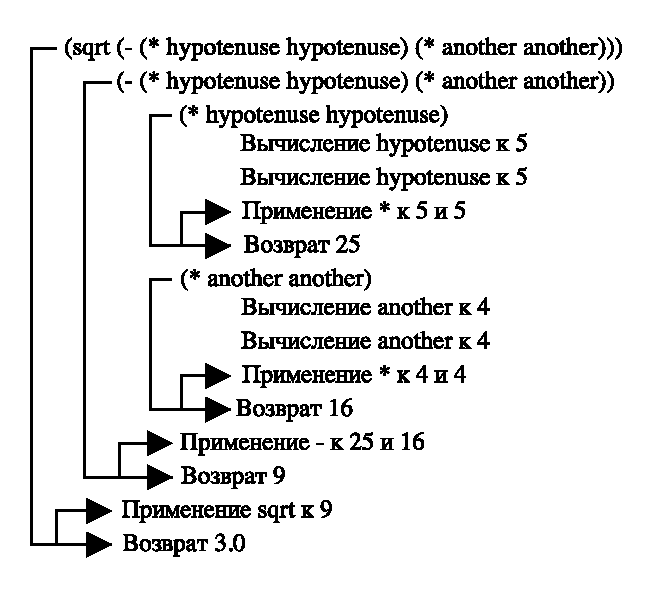
\includegraphics{img/04.pdf}
    \caption{Диаграмма задания 4}
\end{figure}

\section{ЗАДАНИЕ 5}

Написать функцию, вычисляющую площадь трапеции по ее основаниям и
высоте, и составить диаграмму ее вычисления.

\begin{lstlisting}
(defun square (footing1 footing2 height)
    (* (/ (+ footing1 footing2) 2) height)
)

(square 2 2 2) ;;; 4
(square 2 4 5) ;;; 15
\end{lstlisting}

\begin{figure}[H]
    \centering
    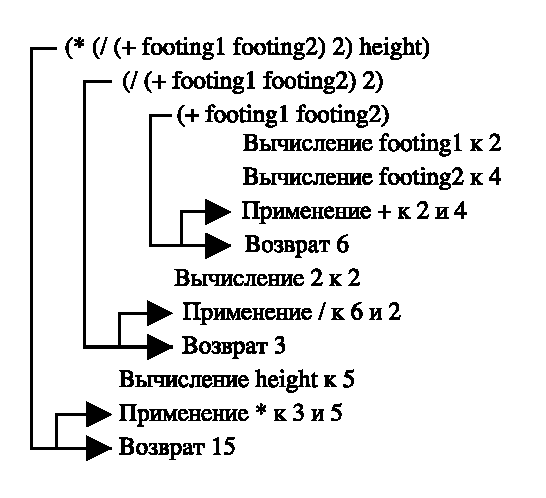
\includegraphics{img/05.pdf}
    \caption{Диаграмма задания 5}
\end{figure}
